\beamersection{Fortgeschrittene Verwendung}

\subsection{Funktionen plotten}

\begin{Frame}{Beispiel eines Funktionsplots}{\texttt{examples/funktionen.tex}}
  \tikzexample{[domain=0:5]
    \draw[very thin,gray] (0,-1.4) grid (4.9,3.4);
    \draw[->] (0,0) -- (5.2,0) node[right] {$x$};
    \draw[->] (0,-1.5) -- (0,3.5) node[above] {$f(x)$};
    %
    \foreach \x in {1,...,4}
      \draw[xshift=\x cm] (0,2pt) -- (0,-2pt) node[below,fill=tikzexample] {$\x$};
    \foreach \y in {-1,...,3}
      \draw[yshift=\y cm] (2pt,0) -- (-2pt,0) node[left,fill=tikzexample] {$\y$};
    %
    \draw[red]    plot (\x,\x/3)         node[right] {$f(x) = \frac{x}{3}$};
    \draw[blue]   plot (\x,{sin(\x r)})  node[right] {$f(x) = \sin x$};
    \draw[orange] plot (\x,{exp(\x)/50}) node[right] {$f(x) = \frac{e^x}{50}$};
  }
\end{Frame}

\begin{Frame}[fragile]{Funktionen plotten}
  \tikzexample{
    \draw[blue,domain=0:5] plot (\x,{sin(\x r)});
    \draw[orange,domain=0:4] plot (\x,{exp(\x)/50});
  }

  \xxx

  \begin{lstlisting}[gobble=4,moretexcs={x}]
    \draw[blue,domain=0:5] plot (\x,{sin(\x r)});
    \draw[orange,domain=0:4] plot (\x,{exp(\x)/50});
  \end{lstlisting}
\end{Frame}

\begin{Frame}[fragile]{Koordinatensystem}
  \tikzexample{
    \draw[very thin,gray] (0,-1.4) grid (4.9,1.4);
    \draw[->] (0,0) -- (5.2,0) node[right] {$x$};
    \draw[->] (0,-1.5) -- (0,1.5) node[above] {$f(x)$};
    %
    \draw[blue,domain=0:5] plot (\x,{sin(\x r)});
    \draw[orange,domain=0:4] plot (\x,{exp(\x)/50});
  }

  \xxx

  \begin{lstlisting}[gobble=4]
    \draw[very thin,gray] (0,-1.4) grid (4.9,1.4);
    \draw[->] (0,0) -- (5.2,0) node[right] {$x$};
    \draw[->] (0,-1.5) -- (0,1.5) node[above]
      {$f(x)$};
  \end{lstlisting}
\end{Frame}

\begin{Frame}[fragile]{Beschriftung der Achsen}
  \tikzexample{
    \draw[very thin,gray] (0,-1.4) grid (4.9,1.4);
    \draw[->] (0,0) -- (5.2,0) node[right] {$x$};
    \draw[->] (0,-1.5) -- (0,1.5) node[above] {$f(x)$};
    %
    \foreach \x in {1,...,4}
      \draw[xshift=\x cm] (0,2pt) -- (0,-2pt) node[below,fill=tikzexample] {$\x$};
    \foreach \y in {-1,...,1}
      \draw[yshift=\y cm] (2pt,0) -- (-2pt,0) node[left,fill=tikzexample] {$\y$};
    %
    \draw[blue,domain=0:5] plot (\x,{sin(\x r)});
    \draw[orange,domain=0:4] plot (\x,{exp(\x)/50});
  }

  \xxx

  \begin{lstlisting}[gobble=4]
    \foreach \x in {1,...,4}
      \draw[xshift=\x cm] (0,2pt) -- (0,-2pt)
        node[below,fill=white] {$\x$};
    \foreach \y in {-1,...,1}
      \draw[yshift=\y cm] (2pt,0) -- (-2pt,0)
        node[left,fill=white] {$\y$};
  \end{lstlisting}
\end{Frame}

\begin{Frame}[fragile]{Beschriftung der Graphen}
  \tikzexample{
    \draw[very thin,gray] (0,-1.4) grid (4.9,1.4);
    \draw[->] (0,0) -- (5.2,0) node[right] {$x$};
    \draw[->] (0,-1.5) -- (0,1.5) node[above] {$f(x)$};
    %
    \foreach \x in {1,...,4}
      \draw[xshift=\x cm] (0,2pt) -- (0,-2pt) node[below,fill=tikzexample] {$\x$};
    \foreach \y in {-1,...,1}
      \draw[yshift=\y cm] (2pt,0) -- (-2pt,0) node[left,fill=tikzexample] {$\y$};
    %
    \draw[blue,domain=0:5] plot (\x,{sin(\x r)}) node[right] {$f(x) = \sin x$};
    \draw[orange,domain=0:4] plot (\x,{exp(\x)/50}) node[right, fill=tikzexample] {$f(x) = \frac{e^x}{50}$};
  }

  \xxx

  \begin{lstlisting}[gobble=4, moretexcs={x}]
    \draw[blue,domain=0:5] plot (\x,{sin(\x r)})
      node[right] {$f(x) = \sin x$};
    \draw[orange,domain=0:4] plot (\x,{exp(\x)/50})
      node[right, fill=white]
        {$f(x) = \frac{e^x}{50}$};
  \end{lstlisting}
\end{Frame}

\subsection{Overlays mit \beamer}

\begin{Frame}{Beispiel von Overlays in Grafiken}{\texttt{examples/tikz-overlays.tex}}
  \tikzexample{[dot/.style={circle,minimum width=5mm,fill=red},
      box/.style={draw, rectangle, inner sep=5mm},
      node distance=4mm and 18mm, thick]
    \uncover<2->{\node[dot] (n1) {};}
    \uncover<3->{\node[dot, right=of n1] (n2) {};}
    \uncover<4->{\node[dot, right=of n2] (n3) {};}
    \uncover<5->{\node[dot, below=of n1] (n4) {};}
    \uncover<6->{\node[dot, below=of n2] (n5) {};}
    \uncover<7->{\node[dot, below=of n3] (n6) {};}
    \node[box, fit=(n1) (n4)] (b1) {};
    \node[box, fit=(n2) (n5)] (b2) {};
    \node[box, fit=(n3) (n6)] (b3) {};
    \node[dot, below=8mm of b1.south west, anchor=west] (r1) {};
    \uncover<1-6>{\node[dot, right=4mm of r1] (r2) {};}
    \uncover<1-5>{\node[dot, right=4mm of r2] (r3) {};}
    \uncover<1-4>{\node[dot, right=4mm of r3] (r4) {};}
    \uncover<1-3>{\node[dot, right=4mm of r4] (r5) {};}
    \uncover<1-2>{\node[dot, right=4mm of r5] (r6) {};}
    \uncover<1>{\node[dot, right=4mm of r6] (r7) {};}
    \node[above=of b2] {$7 \textrm{ mod } 3 = \alt<7>{\alert{1}}{?}$};
  }
\end{Frame}

\begin{Frame}[fragile]{Stile}
  \tikzexample{[dot/.style={circle,minimum width=5mm,fill=red},
      box/.style={draw, rectangle, inner sep=5mm},
      node distance=4mm and 18mm, thick]
    \node[dot] (n1) {};
    \node[box, fit=(n1)] (b1) {};
  }

  \xxx

  \begin{lstlisting}[gobble=4]
    \begin{tikzpicture}[
        dot/.style={circle, minimum width=5mm,
          fill=red},
        box/.style={draw, rectangle,
          inner sep=5mm},
        node distance=4mm and 18mm, thick]
      \node[dot] (n1) {};
      \node[box, fit=(n1)] (b1) {};
    \end{tikzpicture}
  \end{lstlisting}
\end{Frame}

\begin{Frame}[fragile]{Positionierung}
  \begin{lstlisting}[gobble=4]
    \node[dot] (n1) {};
    \node[dot, right=of n1] (n2) {};
    \node[dot, below=of n1] (n4) {};
    % n3, n5, n6
    \node[box, fit=(n1) (n4)] (b1) {};
    % b2, b3
    \node[dot, below=8mm of b1.south west,
      anchor=west] (r1) {};
    % r2, r3, r4, r5, r6
    \node[dot, right=4mm of r6] (r7) {};
  \end{lstlisting}
\end{Frame}

\begin{Frame}[fragile]{Overlays}
  \begin{lstlisting}[gobble=4]
    \uncover<2->{\node[...] (n1) {};}
    % n2, n3, n4, n5
    \uncover<7->{\node[...] (n6) {};}
    \node[box, fit=(n1) (n4)] (b1) {};
    % b2, b3
    \node[dot, below=8mm of b1.south west,
      anchor=west] (r1) {};
    \uncover<1-6>{\node[...] (r2) {};}
    % r3, r4, r5, r6
    \uncover<1>{\node[...] (r7) {};}
  \end{lstlisting}
\end{Frame}

\subsection{Showcase}

\begin{Frame}[shrink]{Computer science mindmap}{Autor: Till Tantau}
  \begin{tikzpicture}
    \path[mindmap,concept color=black,text=white]
      node[concept] {Computer Science}
      [clockwise from=0]
      child[concept color=green!50!black] {
        node[concept] {practical}
        [clockwise from=90]
        child { node[concept] {algorithms} }
        child { node[concept] {data structures} }
        child { node[concept] {pro\-gramming languages} }
        child { node[concept] {software engineer\-ing} }
      }
      child[concept color=blue] {
        node[concept] {applied}
        [clockwise from=-30]
        child { node[concept] {databases} }
        child { node[concept] {WWW} }
      }
      child[concept color=red] { node[concept] {technical} }
      child[concept color=orange] { node[concept] {theoretical} };
  \end{tikzpicture}
\end{Frame}

\begin{Frame}{A family tree}{Autor: Stefan Kottwitz}
  \begin{tikzpicture}[
    man/.style={rectangle,draw,fill=blue!20},
    woman/.style={rectangle,draw,fill=red!20,rounded corners=.8ex},
    grandchild/.style={grow=down,xshift=1em,anchor=west,
      edge from parent path={(\tikzparentnode.south) |- (\tikzchildnode.west)}},
    first/.style={level distance=6ex},
    second/.style={level distance=12ex},
    third/.style={level distance=18ex},
    level 1/.style={sibling distance=5em},thick]
      % Parents
      \coordinate
        child[grow=left] {node[man,anchor=east]{Jim}}
        child[grow=right] {node[woman,anchor=west]{Jane}}
        child[grow=down,level distance=0ex]
      [edge from parent fork down]
      % Children and grandchildren
      child{node[man] {Alfred}
        child[grandchild,first] {node[man]{Joe}}
        child[grandchild,second] {node[woman]{Heather}}
        child[grandchild,third] {node[woman] {Barbara}}}
      child{node[woman] {Berta}
        child[grandchild,first] {node[man]{Howard}}}
      child {node[man] {Charles}}
      child {node[woman]{Doris}
        child[grandchild,first] {node[man]{Nick}}
        child[grandchild,second] {node[woman]{Liz}}};
  \end{tikzpicture}
\end{Frame}

\begin{Frame}{Circuit libraries}{Autor: Till Tantau}
  \begin{tikzpicture}[rotate=-90,circuit ee IEC,x=3.25cm,y=2.25cm]
    %  Let us start with some contacts:
    \foreach \contact/\y in {3/3.5,4/4.5,5/5.5}
    {
      \node [contact] (left contact \contact) at (0,\y) {};
      \node [contact] (right contact \contact) at (1,\y) {};
    }
    \draw (right contact 3)
       -- (right contact 4) -- (right contact 5);
    \draw (left contact 3) -- ++(down:.3) node[left] {\dots};
    \draw (right contact 3) -- ++(down:.3) node[left] {\dots};
    \draw (left contact 3) to [current direction'={near start,info=$\iota$},
                               resistor={near end,info={$R=4\ \Omega$}}]
                           (right contact 3);
    \draw (left contact 4) to [voltage source={near start,
                                               direction info={<-,info={\textrm{8\ V}}}},
                               resistor={info={$2\ \Omega$},near end}] (right contact 4);
    \draw (left contact 3) to [resistor={info={$1\ \Omega$}}] (left contact 4);
    \draw (left contact 4) to [resistor={info={$3\ \Omega$}}] (left contact 5);
    \draw (left contact 5) to [resistor={info={$4\ \Omega$}}] (right contact 5);
    \draw (left contact 5) to [diode] ++(up:1)
                           to [voltage source={near start,
                                               direction info={info={\textrm{3\ V}}}},
                               resistor={near end,info={$3\ \Omega$}}] ++(right:1)
                           to (right contact 5);
  \end{tikzpicture}
\end{Frame}

\begin{Frame}[fragile,shrink]{BER measurement on fibre optical system}{Author: Jose Luis Diaz}
  \only<presentation>{\vspace*{2.5cm}}
  \only<article>{\sideways}
  \begin{tikzpicture}
    % Define a macro to draw the filter symbol
    \newcommand{\filterSS}[1]{\node (#1){};  % This empty node draws the box. 
       % Then we draw the inner curves
       \draw[line width=1pt] (-2mm,-4mm) to[in=200,out=20] (-2mm, 4mm) 
                             (0mm,-4mm) to[in=200,out=20] (0mm, 4mm) 
                             (2mm,-4mm) to[in=200,out=20] (2mm, 4mm); 
       }

    % Define a macro to draw the MOD symbol
    \newcommand{\MOD}[2]{\node (#1) {#2}; % The box with the text inside. Then draw the polygon around the text
      \draw[line width=1pt,sharp corners](-0.75cm,0cm)--(-0.35cm,0.25cm)--
           (0.35cm, 0.25cm)--(0.75cm, 0cm)--(0.35cm, -0.25cm)--(-0.35cm, -0.25cm) -- cycle; 
      }

    % Define a macro to draw the Polariser symbol
    \newcommand{\Polaris}[1]{\node[coordinate] (#1) {}; % Node of type coordinate is a simple point 
         % Now draw the three circles
         \draw[line width=1pt] (0mm, -2mm)  circle (2mm) 
                               (-2mm,2mm)  circle (2mm)
                               (2mm, 2mm)  circle (2mm);}

    % Place all element in a matrix of nodes, called m
    % By default all nodes are rectangles with round corners
    % but some special sytles are defined also
    \matrix (m) [
      column sep=5mm,
      row sep=1cm,
      nodes={draw, % General options for all nodes
        line width=1pt,
        anchor=center, 
        text centered,
        rounded corners,
        minimum width=1.5cm, minimum height=8mm
      }, 
      % Define styles for some special nodes
      right iso/.style={isosceles triangle,scale=0.5,sharp corners, anchor=center, xshift=-4mm},
      left iso/.style={right iso, rotate=180, xshift=-8mm},
      txt/.style={text width=1.5cm,anchor=center},
      ellip/.style={ellipse,scale=0.5},
      empty/.style={draw=none}
      ]
    {
    % First row of symbols (mostly empty, only the power meter at the right end)
      % empty
    & % empty
    & % empty
    & % empty
    & % empty
    & % empty
    & \node[txt] (top power meter) {Power Meter};
    \\

    % Second row of symbols
      \node (laser) {Laser};
    & \MOD{mod}{MOD} 
    & \node[right iso] (iso 1) {};
    & \node (top soa) {SOA};
    & \filterSS{top filter} 
    & \node (top voa) {VOA};
    & \node[ellip] (top connector) {};
    & \node[coordinate, xshift=-1cm] (top right) {};
    \\
    % Third row of symbols
    & \node (mid voa) {VOA};
    & \filterSS{mid filter}  
    & \node[left iso] (iso 2) {};
    & \node[draw=orange!80!white, ultra thick] (qdsoa) {\textbf{QDSOA}};
    & \node[left iso] (iso 3) {};
    & \Polaris{Polaris} 
    & % (no symbol here, only a point to draw the path)
      \node[coordinate, xshift=-1cm] (mid right) {};
    \\
    % Fourth row of symbols
      \node[txt] (low power meter) {Power Meter};
    & \node[ellip] (low ellip) {};
    & \node[right iso] (iso 4) {};
    & \node (low soa) {SOA};
    & \node[right iso] (iso 5) {};
    & \filterSS{low filter} 
    & \node (rx) {Rx};
    & \node[txt] (error detector) {Error\\Detector};
    \\
    };  % End of matrix

    % Now, connect all nodes in a chain.
    % The names of the nodes are automatically generated in the previous matrix. Since the
    % matrix was named ``m'', all nodes have the name m-row-column
    { [start chain,every on chain/.style={join}, every join/.style={line width=1pt}]
      \chainin (laser);
      \chainin (mod);
      \chainin (iso 1);
      \chainin (top soa);
      \chainin (top filter);
      \chainin (top voa);
      % Connect to the power meter, and put a label saying 10%
      \path[line width=1pt] (top power meter) edge node [right] {$10\%$} (top connector);
      \chainin (top connector);
      \chainin (top right);
      % Draw the label saying 90%
      \path (top right) edge node [right] {$90\%$} (mid right) ;
      \chainin (mid right);
      \chainin (Polaris);
      \chainin (iso 3);
      \chainin (qdsoa);
      \chainin (iso 2);
      \chainin (mid filter);
      \chainin (mid voa);
      % Connect to the power meter, and put a label saying 10%
      \path[line width=1pt] (low power meter) edge node [above] {$10\%$} (low ellip);
      \chainin (low ellip);
      % Draw the label saying 90%
      \path (low ellip) edge node [below] {$90\%$} (iso 4) ;
      \chainin (iso 4);
      \chainin (low soa);
      \chainin (iso 5);
      \chainin (low filter);
      \chainin (rx);
      \chainin (error detector);
      };
    % Finally, put some text above some symbols
    \draw (iso 1.left side) node[above, inner sep=5mm] {Isolator};
    \draw (top filter.north) node[above, inner sep=3mm] {Filter};
    \draw (Polaris) node[above, inner sep=6mm, text centered, text width=2cm] {Polarisation\\controller};

    % The big arrow over the MOD symbol is a bit laborious
    \node[yshift=2mm] (MOD arrow) at (mod.north) [anchor=east,single arrow, draw,line width=1pt, 
                  rotate=-90, minimum height=7mm, minimum width=1.3cm, 
                  single arrow head extend=1.2mm, single arrow tip angle=120] {};
    % The text above the arrow (the starting of the arrow is at west in the arrow shape, even if the
    % arrow was rotated and it lies now at top)
    \node (MOD text) at (MOD arrow.west) [above, inner sep=2mm] {10Gb/s PRBS};

    % Define the style for the blue dotted boxes
    \tikzset{blue dotted/.style={draw=blue!50!white, line width=1pt,
                                 dash pattern=on 1pt off 4pt on 6pt off 4pt,
                                  inner sep=4mm, rectangle, rounded corners}};

    % Finally the blue dotted boxes are drawn as nodes fitted to other nodes
    \node (first dotted box) [blue dotted, 
                              fit = (MOD text) (laser) (top soa)] {};
    \node (second dotted box) [blue dotted,
                              fit = (low soa) (error detector)] {};

    % Since these boxes are nodes, it is easy to put text above or below them                          
    \node at (first dotted box.north) [above, inner sep=3mm] {\textbf{Transmitter}};
    \node at (second dotted box.south) [below, inner sep=3mm] {\textbf{Receiver}};
  \end{tikzpicture}
  \only<presentation>{\vspace*{2.5cm}}
  \only<article>{\endsideways}
\end{Frame}

\begin{Frame}[fragile]{Map of a HiSPARC detector}{Autor: David Fokkema}
  \newcommand{\hisparcbox}[1]{%
    \path[hisparc,#1]
        (-.4, .7) .. controls (0, .75) ..  (.4, .7) --
        (.35, -1.7) ..  controls(0, -1.72) ..  (-.35, -1.7) -- cycle;
  }
  \begin{tikzpicture}
    [ x=.5mm, y=.5mm, scale=0.6,
      font={\sffamily},
      station/.style={fill=gray},
      hut/.style={fill=lightgray},
      cluster/.style={fill=yellow!30, rounded corners=2pt},
      road/.style={fill=blue!10},
      calorimeter/.style={fill=green!30},
      tracker/.style={fill=red!30},
      hisparc/.style={fill=red, rounded corners=.15pt},
      hisparcgps/.style={fill=red},
      axis/.style={gray,very thick,->,>=stealth'},
      ruler/.style={gray,|<->|,>=stealth'}
    ]
    % Clusters
    \foreach \i in {-1.5, -0.5, ..., 1.5} {
        \foreach \j in {-1.5, -0.5, ..., 1.5} {
            \path[cluster, shift={(\i * 52, \j * 52)}]
                (-22, -22) rectangle (22, 22);
        }
    }

    % Roads
    \foreach \i in {-1.5, -0.5, ..., 1.5} {
        \path[road, shift={(0, \i * 52 + 2)}]
            (-105, -1.5) rectangle (105, 1.5);
    }

    % Detector array
    \foreach \i in {-7.5, -6.5, ..., 7.5} {
        \foreach \j in {-7.5, -6.5, ..., 7.5} {
            \path[station, shift={(\i * 13, \j * 13)}]
                (-1.2, -1.2) rectangle (1.2, 1.2);
        }
    }
    % Two detectors are slightly displaced
    \path[station, shift={(-6.5, 23.5)}] (-1.2, -1.2) rectangle (1.2, 1.2);
    \path[station, shift={(6.5, 23.5)}] (-1.2, -1.2) rectangle (1.2, 1.2);

    % Electronic huts
    \foreach \i in {-1.5, -0.5, ..., 1.5} {
        \foreach \j in {-1.5, -0.5, ..., 1.5} {
            \path[hut, shift={(\i * 52, \j * 52 - 1.5)}]
                (-2.5, -1.2) rectangle (2.5, 1.2);
        }
    }

    % Central detector
    \fill[white] (-13, -13) rectangle (13, 21);
    \path[calorimeter, shift={(0, 5)}] (-10, -8) rectangle (10, 8);

    % Muon tracker
    \path[tracker, shift={(0, 4)}] (-2.7, 32.5) rectangle (2.7, 70.5);

    % HiSPARC station
    \hisparcbox{shift={(65.0, 15.05)}, rotate=180}
    \hisparcbox{shift={(65.0, 20.82)}, rotate=180}
    \hisparcbox{shift={(70.0, 23.71)}, rotate=-90}
    \hisparcbox{shift={(60.0, 23.71)}, rotate=90}
    \path[hisparcgps, shift={(65.0, 23.71)}] (0, 0) circle (.3);

    % Draw rulers
    \draw[ruler] (-97.5, -105) -- (97.5, -105)
        node[midway,below] {195\ m};
    \draw[ruler] (84.5, 105) -- (97.5, 105)
        node[midway,above] {13\ m};
    \draw[ruler] (-105, -97.5) -- (-105, 97.5)
        node[midway,above,sloped] {195\ m};
    \draw[ruler] (105, 84.5) -- (105, 97.5)
        node[midway,below,sloped] {13\ m};
  \end{tikzpicture}
\end{Frame}

\begin{Frame}[fragile]{Lipid vesicle}{Autor: Henrik Skov Midtiby}
  % Define decoration
  \pgfdeclaredecoration{lipidleaflet}{initial}
  {
    % Place as many segments as possible along the path to decorate
    % the minimum distance between two segments is set to 7 pt.
    \state{initial}[width=\pgfdecoratedpathlength/floor(\pgfdecoratedpathlength/7pt)]
    {
      % Draw the two acyl chains
      \pgfpathmoveto{\pgfpoint{-1pt}{0pt}}
      \pgfpathlineto{\pgfpoint{-1pt}{-10pt}}
      \pgfpathmoveto{\pgfpoint{1pt}{0pt}}
      \pgfpathlineto{\pgfpoint{1pt}{-10pt}}
      % Draw the head group
      \pgfpathmoveto{\pgfpoint{1pt}{0pt}}
      \pgfpathcircle{\pgfpoint{0pt}{2pt}}{2.5pt}
    }
    \state{final}
    {
      \pgfpathmoveto{\pgfpointdecoratedpathlast}
    }
  }

  % Draw a vesicle composed of two lipid layers
  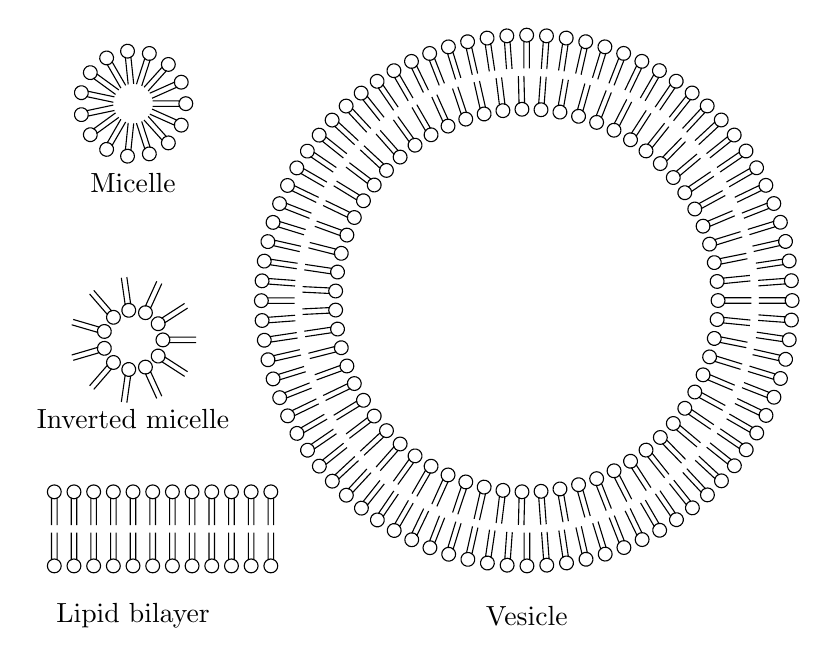
\begin{tikzpicture}
  % Micelle
  \draw[decorate, decoration={lipidleaflet, mirror}] (0, 3) circle (0.6cm);
  \draw (0, 2) node {Micelle};

  % Inverted micelle
  \draw[decorate, decoration={lipidleaflet}] (0, 0) circle (0.45cm);
  \draw (0, -1) node {Inverted micelle};

  % Lipid bilayer
  \draw[decorate, decoration={lipidleaflet, mirror}]
    (-1, -2.8) -- (2, -2.8);
  \draw[decorate, decoration={lipidleaflet}]
    (-1, -2) -- (2, -2);
  \draw (0, -3.5) node {Lipid bilayer};

  % Vesicle
  \draw[decorate, decoration={lipidleaflet}] (5, 0.5) circle (2.5cm);
  \draw[decorate, decoration={lipidleaflet, mirror}] (5, 0.5) circle (3.3cm);
  \draw (5, -3.5) node {Vesicle};

  \end{tikzpicture}
\end{Frame}

\begin{Frame}{Daniell's pile}{Autor: Agustin E. Bolzan}
  \definecolor{copper}{cmyk}{0,0.9,0.9,0.2}
  \colorlet{lightgray}{black!25}
  \colorlet{darkgray}{black!75}
  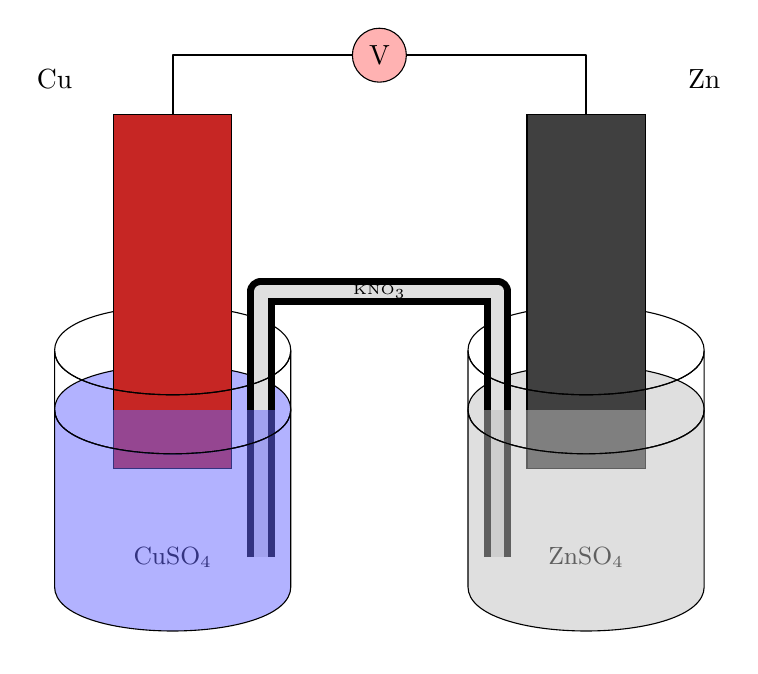
\begin{tikzpicture}[scale=1.5]
    % Draw back of vessel 1
    \draw (0,0) to [controls=+(90:0.5) and +(90:0.5)] (2,0);
    \draw[fill=blue!60, fill opacity=0.5] (0,-0.5) to
        [controls=+(90:0.5) and +(90:0.5)] (2,-0.5);

    % Draw back of vessel 2
    \draw (3.5,0) to [controls=+(90:0.5) and +(90:0.5)] (5.5,0);
    \draw[fill=lightgray, fill opacity=0.5] (3.5,-0.5) to [controls=+(90:0.5)
        and +(90:0.5)] (5.5,-0.5);

    % Draw copper electrode
    \draw[fill=copper] (0.5,2) rectangle (1.5,-1);
    \draw (0,2.3) node {Cu};
    \draw (1,-1.75) node {\small{CuSO$_{4}$}};

    % Draw salt bridge

    \draw[line join=round, line width=10pt] (1.75,-1.75) -- (1.75,0.5) --
        (3.75, 0.5) -- (3.75,-1.75);
    \draw[line join=round, line width=5pt, color=gray!25] (1.75,-1.75) --
        (1.75,0.5) -- (3.75, 0.5) -- (3.75,-1.75);
    \draw (2.75,0.5) node {\tiny{KNO$_{3}$}};

    %Draw front of vessel 1

    \draw (0,0) .. controls +(-90:0.5) and +(-90:0.5) .. (2,0);
    \draw (0,0) .. controls +(-90:0.5) and +(-90:0.5) .. (2,0)
        -- (2,-0.5) .. controls +(-90:0.5) and +(-90:0.5) .. (0,-0.5) -- (0,0);

    %Second part

    \draw[fill=blue!60, fill opacity=0.5] (0,-0.5) .. controls +(-90:0.5)
    and +(-90:0.5) .. (2,-0.5);
    \draw[fill=blue!60, fill opacity=0.5] (0,-0.5) .. controls +(-90:0.5)
    and +(-90:0.5) .. (2,-0.5)
        -- (2,-2) .. controls +(-90:0.5) and +(-90:0.5) .. (0,-2) -- (0,-0.5);

    % draw voltmeter

    \draw[line join=round, thick] (1,2) -- (1,2.5) -- (4.5,2.5) -- (4.5,2);
    \draw (2.75,2.5) node [circle, draw, fill=red!30] {V};

    %Draw back of vessel 2

    %Draw electrode

    \draw[fill=darkgray] (4,2) rectangle (5,-1);
    \draw (5.5,2.3) node {Zn};
    \draw (4.5,-1.75) node {\small{ZnSO$_{4}$}};

    % Draw front of vessel 2
    % part 1
    \draw (3.5,0) .. controls +(-90:0.5) and +(-90:0.5) .. (5.5,0);
    \draw (3.5,0) .. controls +(-90:0.5) and +(-90:0.5) .. (5.5,0)
        -- (5.5,-0.5) .. controls +(-90:0.5) and +(-90:0.5)
        .. (3.5,-0.5) -- (3.5,0);
    % part 2
    \draw[fill=lightgray, fill opacity=0.5] (3.5,-0.5) .. controls +(-90:0.5)
    and +(-90:0.5) .. (5.5,-0.5);
    \draw[fill=lightgray, fill opacity=0.5] (3.5,-0.5) .. controls +(-90:0.5)
        and +(-90:0.5) .. (5.5,-0.5) --
        (5.5,-2) .. controls +(-90:0.5) and +(-90:0.5)
        .. (3.5,-2) -- (3.5,-0.5);
  \end{tikzpicture}
\end{Frame}

\begin{Frame}{Membrane-like surface}{Autor: Yotam Avital}
  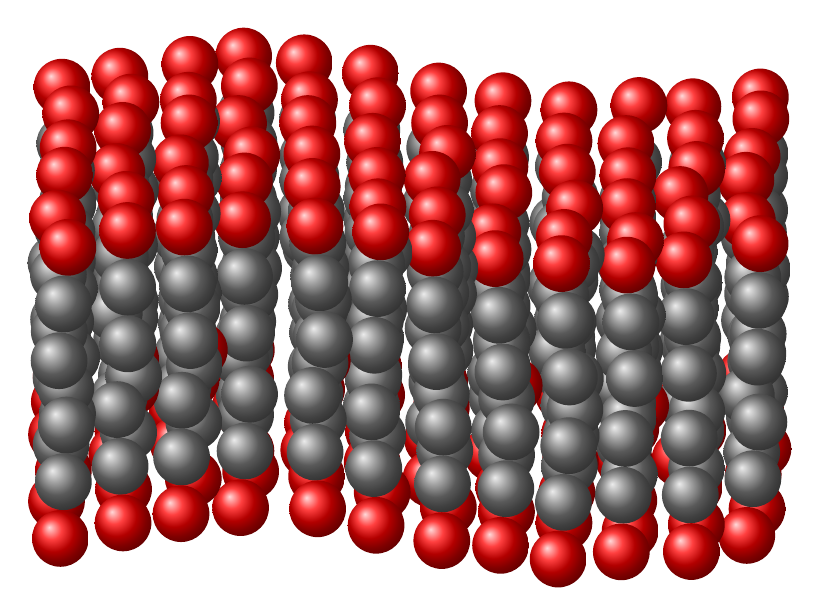
\begin{tikzpicture}[scale=0.8]
    \def\nuPi{3.1459265}
    \foreach \i in {11,10,...,0}{% This one doesn't matter
      \foreach \j in {5,4,...,0}{% This will crate a membrane
                                 % with the front lipids visible
        % top layer
        \pgfmathsetmacro{\dx}{rand*0.1}% A random variance in the x coordinate
        \pgfmathsetmacro{\dy}{rand*0.1}% A random variance in the y coordinate,
                                       % gives a hight fill to the lipid
        \pgfmathsetmacro{\rot}{rand*0.1}% A random variance in the
                                        % molecule orientation
        \shade[ball color=red] ({\i+\dx+\rot},{0.5*\j+\dy+0.4*sin(\i*\nuPi*10)}) circle(0.45);
        \shade[ball color=gray] (\i+\dx,{0.5*\j+\dy+0.4*sin(\i*\nuPi*10)-0.9}) circle(0.45);
        \shade[ball color=gray] (\i+\dx-\rot,{0.5*\j+\dy+0.4*sin(\i*\nuPi*10)-1.8}) circle(0.45);
        % bottom layer
        \pgfmathsetmacro{\dx}{rand*0.1}
        \pgfmathsetmacro{\dy}{rand*0.1}
        \pgfmathsetmacro{\rot}{rand*0.1}
        \shade[ball color=gray] (\i+\dx+\rot,{0.5*\j+\dy+0.4*sin(\i*\nuPi*10)-2.8}) circle(0.45);
        \shade[ball color=gray] (\i+\dx,{0.5*\j+\dy+0.4*sin(\i*\nuPi*10)-3.7}) circle(0.45);
        \shade[ball color=red] (\i+\dx-\rot,{0.5*\j+\dy+0.4*sin(\i*\nuPi*10)-4.6}) circle(0.45);
      }
    }
  \end{tikzpicture}
\end{Frame}

\begin{Frame}[fragile]{Christmas fractal tree}{Autor: Andrew Stacey}
  \tikzset{
    tinsel/.style={
      #1,
      rounded corners=10mm,
      ultra thin,
      decorate,
      decoration={
        snake,
        amplitude=.1mm,
        segment length=10,
      }
    },
    baubles/.style={
      decorate,
      decoration={
        markings,
        mark=between positions .3 and 1 step 2cm
        with
        {
          \pgfmathsetmacro{\brad}{2 + .5 * rand}
          \path[shading=ball,ball color=#1] (0,0) circle[radius=\brad mm];
        }
      }
    },
    lights/.style={
      decorate,
      decoration={
        markings,
        mark=between positions 0 and 1 step 1cm
        with
        {
          \pgfmathsetmacro{\tint}{100*rnd}
          \node[rotate=90,dart,shading=ball,inner sep=1pt,ball color=red!\tint!yellow] {};
        }
      }
    }
  }
  \qquad
  \begin{tikzpicture}[scale=0.8]
    \coordinate (star) at (0,-1);
    \path (star) +(-50:7) coordinate (rhs) +(-130:7) coordinate (lhs);
    \draw[brown!50!black,line width=5mm,line cap=round] (star) ++(-90:6.8) -- ++(0,-1) coordinate (base);
    \node[scale=-1,trapezium,fill=black,minimum size=1cm] at (base) {};
    \foreach \height/\colour in {%
      .2/blue,
      .4/yellow,
      .6/red,
      .8/orange,
      1/pink%
    } {
      \draw[tinsel=\colour] ($(star)!\height!(lhs)$) to[bend right] ($(star)!\height!(rhs)$);
    }
    \path (star);
    \pgfgetlastxy{\starx}{\stary}
    \begin{scope}[xshift=\starx,yshift=\stary,yshift=-7cm]
    \draw[color=green!50!black, l-system={rule set={S -> [+++G][---G]TS,  G -> +H[-G]L, H -> -G[+H]L, T -> TL, L -> [-FFF][+FFF]F}, step=4pt, angle=18, axiom=+++++SLFFF, order=11}] lindenmayer system -- cycle;
    \end{scope}
    \foreach \height/\colour in {%
      .1/pink,
      .3/red,
      .5/yellow,
      .7/blue,
      .9/orange%
    } {
      \draw[tinsel=\colour] ($(star)!\height!(lhs)$) to[bend right] ($(star)!\height!(rhs)$);
    }
    \foreach \height in {.15,.35,...,1} {
      \draw[lights] ($(star)!\height!(lhs)$) to[bend right] ($(star)!\height!(rhs)$);
    }
    \foreach \angle/\colour in {
      -50/red,
      -70/yellow,
      -90/blue,
      -110/pink,
      -130/purple%
    } {
      \draw[baubles=\colour] (star) -- ++(\angle:7);
    }
    \node[star,star point ratio=2.5,fill=yellow,minimum size=1cm] at (star) {};
  \end{tikzpicture}
\end{Frame}

